\section{Black box modeling approach}

% Motivation for a black box model of the complete circuit
The goal of the black-box modeling method is to build a combined electrical and failure model of an integrated function between two external pins.
This model is developped to allow third-parties that don't have access to the integrated circuit design to perform ESD simulations of a board containing integrated circuits.
The electrical part of the model serves to run the \gls{spice} simulations.
The failure part of the model watches the external input pin and detects conditions that would lead to a failure visible on the external output pin.
The black box model is intented to act as a replacement for the \gls{ic} function during \gls{esd} board-level simulations.
This approach follows the recommendation of the \gls{seed} methodology \cite{seed} presented earlier.
The \gls{seed} methodology normally applies to hard-failure, but in this chapter the concept is pushed further with soft-failures.
\gls{seed} recommends that the ESD robustness of a system should be handled by a collaboration between the board and the integrated circuit.
To achieve this, it is necessary to have simulation tools capable of simulating both elements at the same time.
The black-box model presented in this chapter is a potential solution to this issue.
It does not reveal the internal IC design while allowing complete simulations of board and integrated circuits together to predict soft-failures.
It also abstracts the internal complexity of the integrated circuit design, allowing significantly faster simulations and less convergence issues.

% What is the model
As previously described, the two requirements for the model is to be usable in \gls{spice} simulations and to detect failures by monitoring the input.
This can be achieved with a model containing a failure element and two electrical models as proposed in Fig. \ref{fig:black-box-principle}.
The input port model reproduces the behavior of the integrated circuit between the external input pin and (usually) a ground pin.
The failure model watches for voltage or current on the input port, compares those parameters to the failure characterization and deduces if the input was sufficiently disturbed to create a fault.
Then, it transfer that information to the output port model, that changes behavior in case of fault or remains in its DC state in the absence of a failure.

\begin{figure}[!h]
  \centering
  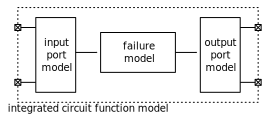
\includegraphics[width=0.65\textwidth]{src/4/figures/black_box_model_principle.pdf}
  \caption{Black-box model principle}
  \label{fig:black-box-principle}
\end{figure}

% How is the model constructed
The failure model is extracted first, using a set of variable amplitude and variable width rectangular pulses applied on the input pin while monitoring the output pin.
After this step, the robustness of the function against this range of stresses is known.
A curve is built that describes the failure of the output when an input is stressed.
The second step is to electrically model both the input and the output ports.
Initially, a \gls{tlp} characterization of each port is performed to extract an equivalent I(V) curve.
Since the circuit is stressed while being powered and in operation, it is studied afterward if this extraction should occur on a device powered as well or not, and what is the impact of the supply on the extracted curve.
This characterization is based on the hypothesis that the quasi-static I(V) curve could be suitable for reproducing the behavior of the port both in DC and transient domain.
It will be demonstrated afterward that this hypothesis is not completely true and an alternative approach is required for the output pin.
This I(V) curve is converted in an electrical model using a piecewise-linear curve described in Verilog-A modelling language.
Finally, once the two electrical models and the failure model have been constructed, it can be possible to join all the parts together to build the complete IC model.

% Detail the particular simulation process
%TODO
The process to simulate an entire board following SEED is the following
A SPICE simulation with the input port model is ran
After the simulation, the input curve is analysed to see if an failure will occurr on the output.
Then, a second simulation is ran with the output setup this time.
If the failure was detected in the first, the info is passed to the output model that generates a fake failure ressembling the one measured.
At the end of this process, a board simulation could be ran to simulate the behavior of the IC.
It is not as straightforward as a single simulation but it can already achieve the SEED goal.

The concept was not tested entirely in simulation because of some issues discovered late, but using a particular setup it is possible to build it as follow-up work.
The next part of this chapter details further the modelling approach and all the issues met during the developpement as well as possible improvements.
% END TODO

% What is the case study
To validate the concept, the characterization is performed on the integrated primary supply studied earlier (see Chapter \ref{sec:supply-desc}).
The input pin is called $V_{batt}$ and accepts the battery supply voltage.
The output pin is called $V_{2p5}$ and is supposed to deliver a 2.5V regulated supply.
Fig. \ref{fig:black-box-applied} summarize the model configuration with those pins and function.

\begin{figure}[!h]
  \centering
  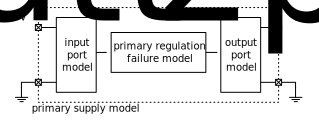
\includegraphics[width=0.65\textwidth]{src/4/figures/black_box_model_applied.pdf}
  \caption{Black-box model applied to the primary regulation function}
  \label{fig:black-box-applied}
\end{figure}


\subsection{Function failure model}

% First the function failure is characterized
As previously detailled, the primary regulation function failure is characterized first.
This is done by applying a set of variable width and variable amplitude rectangular pulses on the input pin, while monitoring the behavior of the output pin.
In case of significant variations of behavior, a failure is recorded.
The characterization yields a lookup table (see Table \ref{tab:cz-failure}) that associates to an input width and an input amplitude a flag representing the presence or absence of a failure.

\begin{table}[!h]
\centering
\begin{tabular}{@{}lll@{}}
\toprule
input width (ns) & input amplitude (V) & Failure   \\ \midrule
10               & 1                   & No        \\
10               & 2                   & No        \\
etc.             & ...                 & ...       \\
100              & 1                   & No        \\
etc.             & ...                 & ...       \\
1000             & 10                  & Yes       \\
etc.             & ...                 & ... \\ \bottomrule
\end{tabular}
\caption{Example of resulting table of failure characterization}
\label{tab:cz-failure}
\end{table}

% How is the characterization conducted and with which values
The characterization pulses are injected on the $V_{batt}$ input.
If a voltage below 2.1V is detected on $V_{2p5}$, a failure is recorded.
This voltage threshold is the failure criteria.
This value was chosen because it corresponds to a level below which digital cells powered by this supply will have noise margins too small for proper operation.
The input stress amplitude range is from -50 V to -500 V.
The input stress width is comprised between 1 ns and 1000 ns.
The characterization setup is given in Fig. \ref{fig:cz-black-box-setup}.
On the input pin, a 12 V bias supply is connected in series with the rectangular pulse generator.
On the output, a 100 nF capacitor is connected because required by the regulation function for stabilisation.

\begin{figure}[!h]
  \centering
  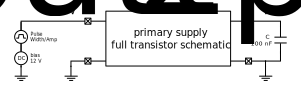
\includegraphics[width=0.7\textwidth]{src/4/figures/black_box_model_setup.pdf}
  \caption{Black-box characterization setup}
  \label{fig:cz-black-box-setup}
\end{figure}

% Detail the characterization
The result of the characterization is plotted in Fig. \ref{fig:cz-black-box}.
The x-axis is the pulse width, the y-axis is pulse amplitude and a colored cell represents a failure on the output.
This plot is simply a different representation of the lookup table discussed previously.
The plot shows that a combination of long stresses and large amplitude are the most disturbing for the function.
Amplitude or width alone are not necessarily sufficient to put the function at fault.

\begin{figure}[!h]
  \centering
  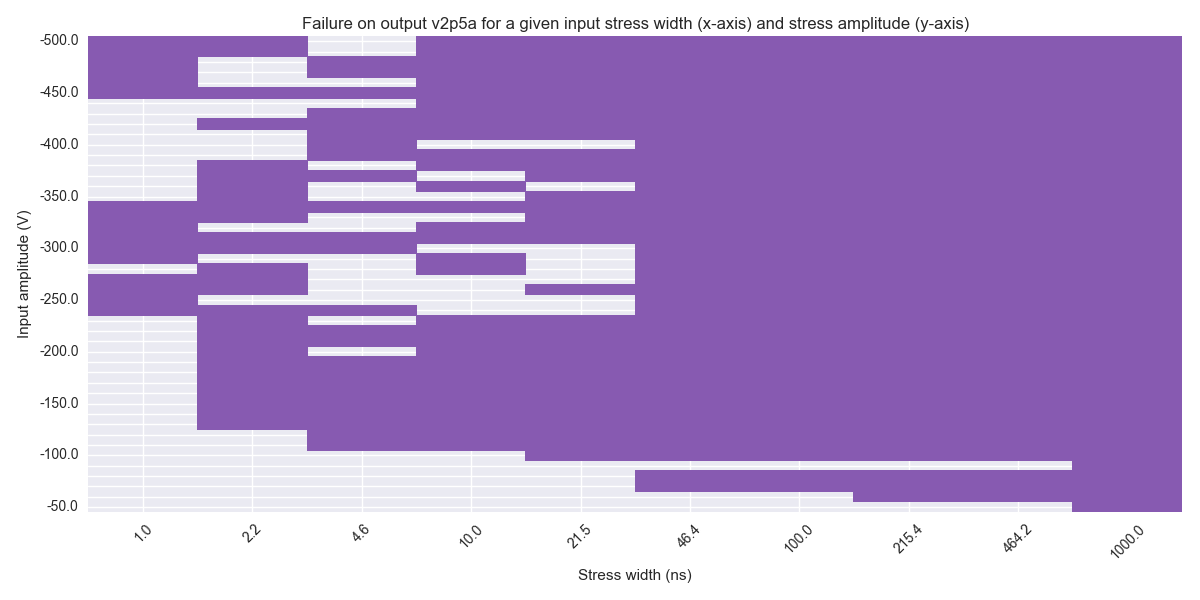
\includegraphics[width=\textwidth]{src/4/figures/black_box_regulator.png}
  \caption{Black-box characterization of the regulation function}
  \label{fig:cz-black-box}
\end{figure}

Now that the characterization step is done, the next part of this work focuses on electrical modelling of input and output pins.

\subsection{Electrical pin models}
\subsubsection{I(V) curve extraction in powered and unpowered modes}

% powered or unpowered conditions ?
As a remainder, they initial hypothesis in this section is that \gls{tlp} characterization can be used to represent an input or output port of an integrated function.
Extracting the \gls{tlp} characteristic can be done with the device powered or unpowered.
To see the impact of the biasing and decide the best approach, \gls{tlp} characterizations are performed in both conditions.
The test setup for the input port is given in Fig. \ref{fig:tlp-input-testbench}.
The DC source can be configured for 0 V supply (unpowered conditions) or 12 V (powered conditions).
The TLP is a perfect rectangular source in combination with a series 50 \textOmega{} resistor.

\begin{figure}[!h]
  \centering
  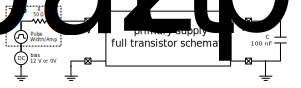
\includegraphics[width=0.8\textwidth]{src/4/figures/black_box_model_tlp_setup.pdf}
  \caption{I(V) extraction of input port}
  \label{fig:tlp-input-testbench}
\end{figure}

The test setup for the output port is given in Fig. \ref{fig:tlp-output-testbench}.
The main issue with this characterization is that it includes the external stabilisation capacitor.
It will be verified after if this external device is an issue for modelling.

\begin{figure}[!h]
  \centering
  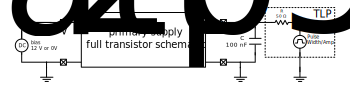
\includegraphics[width=0.9\textwidth]{src/4/figures/black_box_model_tlp_setup_output.pdf}
  \caption{I(V) extraction of output port}
  \label{fig:tlp-output-testbench}
\end{figure}

The results are provided for the input and output ports in Fig. \ref{fig:tlp-input-cz} and \ref{fig:tlp-output-cz}.

\begin{figure}[!h]
  \centering
  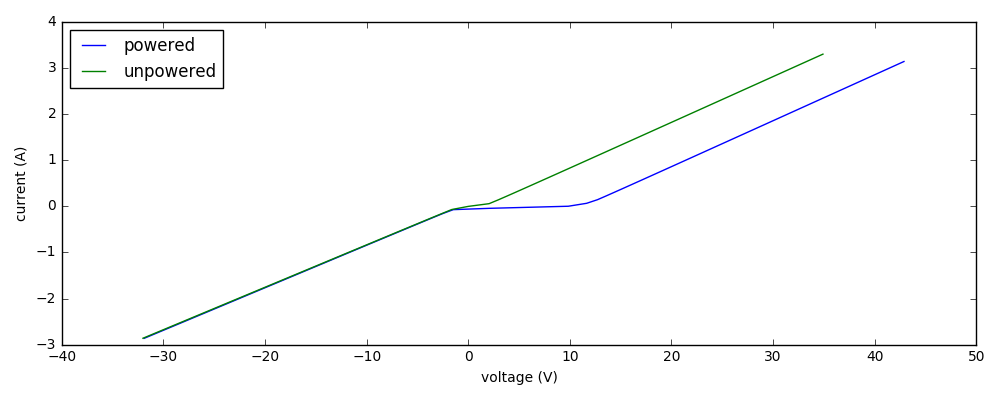
\includegraphics[width=\textwidth]{src/4/figures/tlp_input_characterization.png}
  \caption{TLP characterization of function input in powered and unpowered conditions}
  \label{fig:tlp-input-cz}
\end{figure}

\begin{figure}[!h]
  \centering
  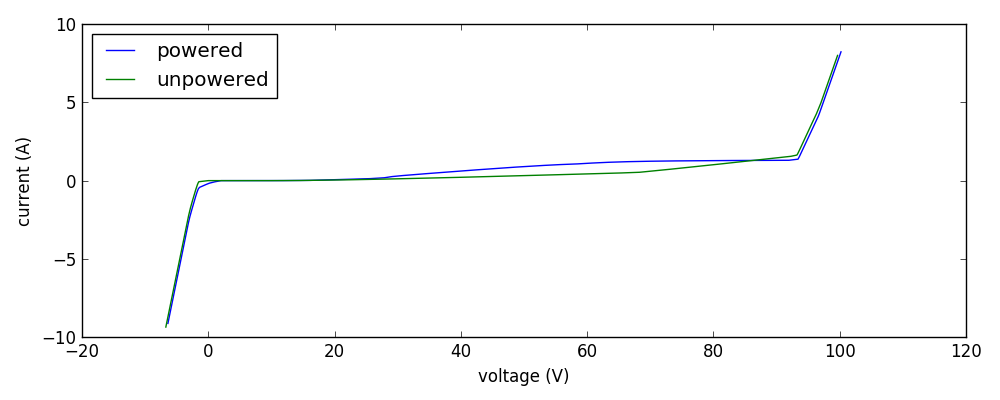
\includegraphics[width=\textwidth]{src/4/figures/tlp_output_characterization.png}
  \caption{TLP characterization of function output in powered and unpowered conditions}
  \label{fig:tlp-output-cz}
\end{figure}

% Comment the results
For both ports, large differences are observed between powered and unpowered modes.
Different amount of currents are absorbed by the device in each conditions.
Ultimately, the powered configuration is chosen for the characterization because it is the one used for soft-failure testing (with the device in operation).

\subsubsection{I(V) curve modelling}

% Explain the PWL model
The second step of the modelling method is to build an electrical model of the function from those curves.
A piecewise linear model seems well suited for this situation.
A four-points piecewise linear model is written in Verilog-A (see Listing \ref{lst:pwl-4pts}).
The model is configured easily with 4 four (V\textsubscript{i},I\textsubscript{i}) coordinates.

\begin{code}
\inputminted[frame=single]{verilog}{src/4/snippets/pwl_4pts.va}
\caption{Piecewise linear 4-points Verilog-A model}
\label{lst:pwl-4pts}
\end{code}

% How to avoid convergence issues
With this kind of model, convergence can be difficult to achieve if the piecewise-linear curve is not continuous at order 0.
Electrically speaking, it is equivalent to switching the value of a resistor very abruptly.
To ensure that this does not happen, it is important to use \textbr{exactly} the same coordinates at inflexion points, where the model switches between operating curves.
This is taken into account in the current model.

% Focus on the area of interest
During this \gls{tlp} characterization, I(V) curves were extracted for a wide range of voltages.
However, not the entire I(V) curve is relevant for those soft-failure simulations.
Any part of the I(V) curve beyond the safe operating area is irrelevant because after that the function is destroyed.
Therefore, it is important to fit the I(V) curve with the piecewise linear curve inside the SOA.
For the input, the modelling is focused on a voltage range from -10V to 40V.
On the output, the modelling range is from -5V to 5V.

\subsubsection{Comparison of input model with reference circuit}

% Validate the model with TLP
The Verilog-A model is tested against the complete schematic for the function's input.
The test setup is given in Fig. \ref{fig:compare-veriloga-model-input}.
Biasing and injection circuits are identical for both circuits.
The full schematic is simply replaced by the Verilog-A input model.

\begin{figure}[!h]
  \centering
  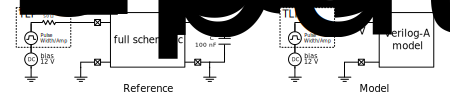
\includegraphics[width=0.95\textwidth]{src/4/figures/testbench_blackbox_input.pdf}
  \caption{Testbench for comparing complete schematic with input model simulations}
  \label{fig:compare-veriloga-model-input}
\end{figure}

% What is the result of comparison of model versus complete schematic for input ?
A first comparison is ran by injecting a -10V TLP with the device powered.
The voltage and current waveforms are provided in Fig. \ref{fig:compare-model-simu-m10}.
Voltage matches well between the reference and the Verilog-A model.
The DC behavior as well as the transient behavior are correctly reproduced.
The current waveform has a poorer correlation.
There is an offset in DC and in transient, probably due to a modelling error with the piecewise linear curve.
There are two large spikes at the beginning and the end of the pulse that are not reproduced.
This behavior was expected because the piecewise-linear model is not able to reproduce this kind of dynamic behavior.
Overall, the accuracy remains acceptable for an ESD simulation.

Other validations are provided for positive 20V and 40V TLP in Fig. \ref{fig:compare-model-simu-20} and Fig. \ref{fig:compare-model-simu-40}).
They confirm that the input model performs correctly, and even better when exposed to positive stresses.
Overall, this Verilog-A model is considered valid for the input port while considering that there is a lot of room for improvement.

\begin{figure}[!p]
  \centering
  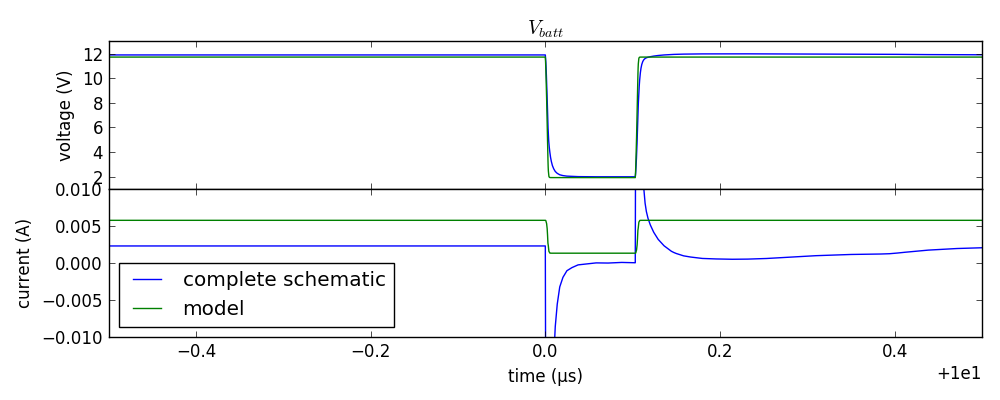
\includegraphics[width=0.8\textwidth]{src/4/figures/comparison_model_total_m10V.png}
  \caption{Comparison of complete schematic and model simulations for input port (-10V TLP)}
  \label{fig:compare-model-simu-m10}
\end{figure}

\begin{figure}[!p]
  \centering
  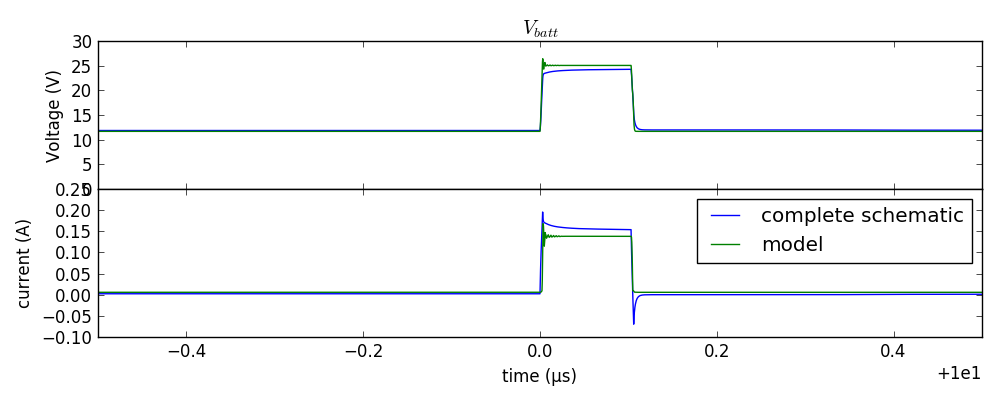
\includegraphics[width=0.8\textwidth]{src/4/figures/comparison_model_total_20V.png}
  \caption{Comparison of complete schematic and model simulations for input port (20V TLP)}
  \label{fig:compare-model-simu-20}
\end{figure}

\begin{figure}[!p]
  \centering
  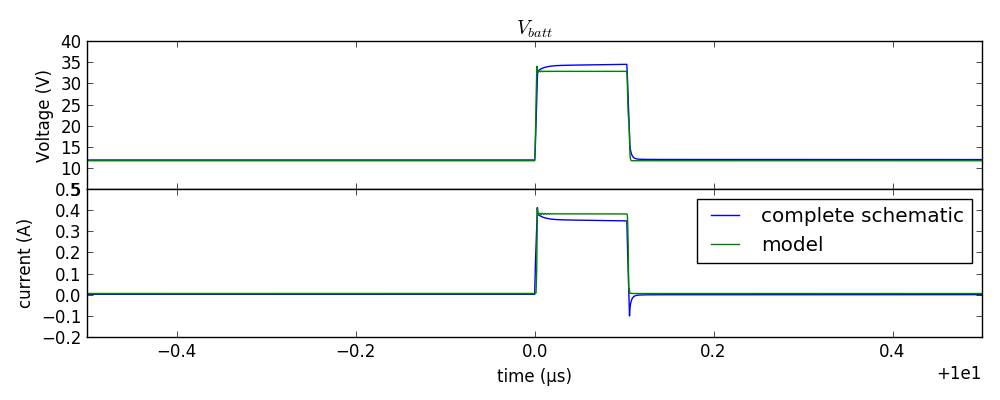
\includegraphics[width=0.8\textwidth]{src/4/figures/comparison_model_total_40V.png}
  \caption{Comparison of complete schematic and model simulations for input port (40V TLP)}
  \label{fig:compare-model-simu-40}
\end{figure}

\subsubsection{Comparison of output model with reference circuit}

% The output port is not a passive device
The output port is more complicated than the input port, because it is equivalent to an active device, unlike the input that can be assimilated to a passive port.
The primary supply regulates a 2.5 V voltage on this output and drives a current into the external load to maintain that voltage.
The Verilog-A I(V) model used for the input is just a voltage controlled current source and is not capable of regulating a voltage.
A more complex architecture is proposed with Fig. \ref{fig:first-output-model}.
A DC voltage source is added to generate the regulated 2.5V.
In case of failure, the output port will also fail temporarily and the output voltage will fall down.
A transient voltage source is added to the model to simulate the output fault.

\begin{figure}[!h]
  \centering
  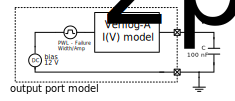
\includegraphics[width=0.7\textwidth]{src/4/figures/first_output_model.pdf}
  \caption{Architecture of the output port model}
  \label{fig:first-output-model}
\end{figure}

% Make the comparison
This new output port model is compared to the complete schematic in simulation.
With the complete schematic, a failure is triggered by applying a negative -10V TLP on the input port $V_{batt}$ while watching the output $V_{2p5}$.
For the model, the PWL source is used to fake a failure.
The testbench is identical to the input validation testbench shown previously (Fig. \ref{fig:compare-veriloga-model-input}).
Voltage and current waveforms are compared in Fig. \ref{fig:compare-model-simu-m10-output}.

\begin{figure}[!h]
  \centering
  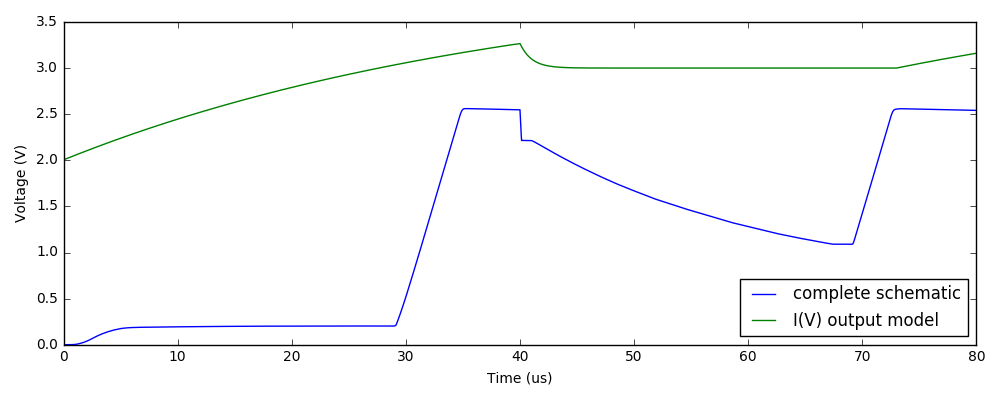
\includegraphics[width=\textwidth]{src/4/figures/comparison_model_total_output_bad_m10V.png}
  \caption{Comparison of complete schematic and model simulations for output port (-10V TLP)}
  \label{fig:compare-model-simu-m10-output}
\end{figure}

% Comment the reference curve
Large differences are observed between reference and model simulations.
In the reference curve (in blue), the regulation is starting up between 0 and 35\textmu{}s.
This part of the curve is not particularly relevant for the ESD analysis and can be ignored overall.
Then, at 40\textmu{}s, the pulse is injected on the input (not plotted), resulting in a fault on this output.
In turn, the reference curve exhibits the typical restart explained previously in chapter \ref{sec:failure-case-study}.
The voltage drops until 1V, then the regulator restarts until it is operating properly again at 75 \textmu{}s.

% Comment the model curve
The model curve (in green) is very different from the reference.
Initially, the 100nF capacitor connected on the output (Fig. \ref{fig:first-output-model}) is pre-charged at 2V, to see if the model is capable of charging it at 2.5V and reaching the DC operating point.
Instead, the output voltage keeps increasing.
This can be explained by looking at the I(V) curve of the output magnified between 1V and 4V (see Fig. \ref{fig:tlp-output-cz-zoomed}).
At the beginning of the simulation, the I(V) model sees a potential difference of 2.0V accross its terminals.
For a 2.0V voltage, the I(V) curve model produces a value of 0.75 mA.
It is not identical to the characterized value of 0.2mA but the error remains acceptable.
This non-zero current is therefore forced by the Verilog-A model into the the capacitor, that keeps charging.
In itself, the
The combination of the DC source and the I(V) curve does not seem suitable for modelling an active output.

\begin{figure}[!h]
  \centering
  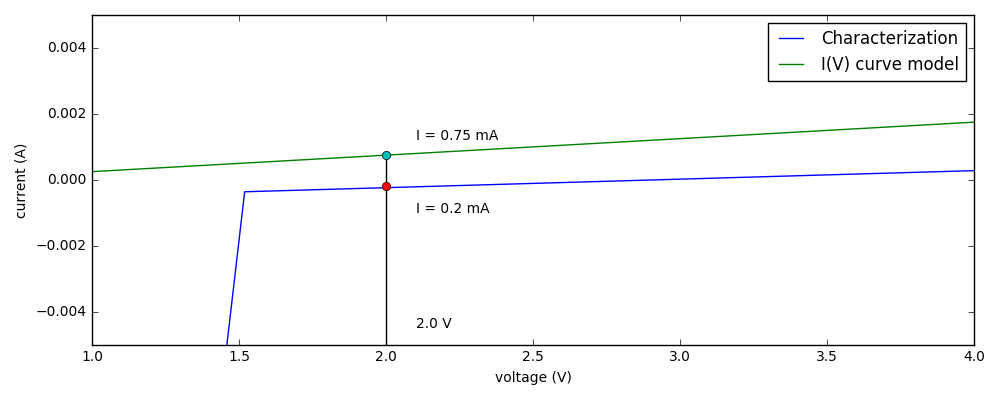
\includegraphics[width=\textwidth]{src/4/figures/tlp_output_characterization_magnified.png}
  \caption{TLP characterization of function output near 2.5V (magnified)}
  \label{fig:tlp-output-cz-zoomed}
\end{figure}

Configuring the Verliog-A model to generate a zero current at 2.5 V will not solve the problem either because with a resistive load the output will need to supply a DC current at 2.5V.
The I(V) curve extracted with a TLP characterization in simulation does not seem to be usable as-is to model an active output.
A more complex or different solution must be conceived and developped to solve those issues.
One potential solution would be to create a custom Verilog-A model capable of regulating a voltage while offering proper output impedance.
Overall, this study on input and output ports modelling has enabled to identify key issues preventing for now to develop a complete model of integrated function for powered ESD simulations.
This is a first step toward more advanced models and modelling techiques that ultimately should enable better cooperation between silicon-design companies and equipment manufacturers, as described by the SEED methodology.

\subsection{Conclusion on black-box modeling}


% Conclusion
Black box models are very promising for distributing SPICE models of integrated functions to third-parties without disclosing intellectual property.
They do not disclose the internal design of the chip and might help achieve system-level ESD simulations with IC models.
Ultimately, the goal is to follow the SEED \cite{seed} methodology that indicates that ESD robustness of a system should not be handled by a single component but with a collaboration between all parts (equipment, board, integrated circuit), using appropriate design techniques to ensure that the cooperation is efficient.
In this section, a first attempt at extracting and creating black-box models for integrated functions was presented, in the context of ESD simulations.
TLP characterization was performed on input and ouput pin of a biased function, to extract an equivalent impedance.
The resulting I(V) curve was then modelled using Verilog-A modelling language, then used in circuit simulations.
For the input pin that is somehow equivalent to a passive device, this model has shown promising results with excellent correlation in both DC and transient domains.
The Verilog-A model performed particularly good for the input when expositive to a positive rectangular stress.
The correlation was less accurate with a negative rectangular pulse but remained acceptable for an ESD simulation.
For the output pin, the situation was more complex because it should be modelled by an equivalent active device.
A first model was proposed specifically for modelling active outputs, however it was not successful.
Differences between the reference schematic and the model were simply too large, showing that a different or more complex approach is required.
Despite the lack of correlation, this study has enabled to identify a important issue preventing to build a model of an integrated function, for ESD simulations.
Solving this issue should be the topic for future work and research, and identifying it was already a significant milestone to reach for achieving this goal.
Ultimately, black box models should enable to replace a integrated function during an ESD simulation, in order to reduce complexity, simulation time, and protect intellectual property.

% Opening work
There are many new leads to explore on these black box models, and work to accomplish.
The behavior of the black-box models should be investigated against more time-varying disturbances such as ESD gun waveforms.
The piecewise-linear modelling technique, usually employed in the ESD field for modelling ESD protections, should be improved to be more stable and fit more closely the extracted I(V) curve.
The methodology should be applied to a wider number of analog functions, to observe if it can be used in a general manner.
For now, input and outputs must be simulated separately.
First, the input is simulated, then analyzed to extract the width and amplitude of the disturbance.
This data is then used to configure the output failure source pulse.
The model must be improved in order for the output to react in real-time to the disturbance of the input.
Research on all those topics should lead to the development a black-box model that will work for powered electrostatic discharge simulations.
